\documentclass[t]{beamer}

\usetheme[compress]{Dresden}
%\usecolortheme{beaver}
\usefonttheme{professionalfonts}
% Insert the frame number at the bottom line
\expandafter\def\expandafter\insertshorttitle\expandafter{%
  \insertshorttitle\hfill\insertframenumber\,/\,\inserttotalframenumber}
% Remove the navigation symbols (one of the two options)
%\usenavigationsymbolstemplate{}
\setbeamertemplate{navigation symbols}{}

\usepackage{graphicx,color,dashbox,amsmath}
\usepackage{hyperref}% embedding hyperlinks [must be loaded after dropping]
\usepackage{amsmath}
\usepackage{amsthm,amssymb,amsfonts,latexsym,mathrsfs,wasysym}
\usepackage{pifont}
\usepackage{marvosym}
\usepackage{subfigure}
\usepackage{epstopdf}
\usepackage{soul,color}
\usepackage{threeparttable}% tables with footnotes
\usepackage{dcolumn}% decimal-aligned tabular math columns
\usepackage{float}
\usepackage{algorithm}
\usepackage[noend]{algpseudocode}
%\usepackage{subfig}

%\usepackage[style=ieee,backend=bibtex,citestyle=ieee]{biblatex}
%\usepackage[multiple]{footmisc}
%\addbibresource{bibliography.bib}
%\usepackage{colortbl}

\usepackage{tikz}
\usetikzlibrary{calc}
\usetikzlibrary{shapes.geometric}
\usetikzlibrary{arrows.meta}

%\usepackage{enumitem}
%\newlist{arrowlist}{itemize}{1}
%\setlist[arrowlist]{label=$\Rightarrow$}

\newcolumntype{d}{D{.}{.}{-1}}
\graphicspath{{Figures/}}

\logo{
\includegraphics[width=3em]{lapid-logo-45}}
\renewcommand{\baselinestretch}{1.2}

% commands and colors
\newcommand{\rR}{\mathbb{R}}
\newcommand{\rsqr}{\mathbb{R}^2}
\newcommand{\rthrd}{\mathbb{R}^3}
\newcommand{\eqsn}[1]{\begin{equation}#1\end{equation}}
\newcommand{\br}{$\\ $}

\newcommand{\bmat}[1]{\begin{bmatrix}#1\end{bmatrix}}
\newcommand{\mat}[1]{\begin{matrix}#1\end{matrix}}
\newcommand{\vmat}[1]{\begin{vmatrix}#1\end{vmatrix}}

\newcommand{\con}{c\left(t\right)}
\newcommand{\conp}[1]{c_{#1}\left(t\right)}
\newcommand{\concov}{\mathtt{C}\left(\con\right)}
\newcommand{\concovp}[1]{\mathtt{C}\left(\conp{#1}\right)}
\newcommand{\conset}{\mathtt{G}}

\newcommand{\sigp}{\sigma\left(p\right)}
\newcommand{\sigpp}[2]{\sigma_{#1 #2}\left(p \right)}
\newcommand{\pb}{\bar{p}}

\newcommand{\norm}[1]{\lVert #1 \rVert}

\makeatletter
\newcommand{\mathleft}{\@fleqntrue\@mathmargin0pt}
\newcommand{\mathcenter}{\@fleqnfalse}
\makeatother


% Gilad New Commands
\newcommand{\sgn}[1]{\operatorname{sgn}\left(#1\right)}
\newcommand{\sat}[1]{\operatorname{sat}\left(#1\right)}
%\newcommand{\rrule}[1]{\rule[#1]{0pt}{0pt}}

%beamer@blendedblue
\definecolor{mgreen}{RGB}{40,160,40}
\definecolor{natigreen}{RGB}{50,205,50}
\definecolor{natiblue}{RGB}{0,191,255}
\definecolor{mg}{rgb}{0,0.4,0}%
\definecolor{mypink2}{RGB}{219, 48, 122}

\newtheorem*{Proposition}{Proposition}
\newtheorem*{keylemma}{Key Lemma}
\newtheorem*{Remark}{Remark}
\newtheorem*{question}{Question}
\newtheorem*{Task}{Task}
\newtheorem*{cor}{Corollary}
\newtheorem*{thm}{Theorem}



%%%%%%%%%%%%%%%%%%%%%%%%%%

\title{A Projected Lloyd’s Algorithm for Coverage Control Problems}

\author
{Yoav Palti, Supervisor: Associate Professor Daniel Zelazo}

\institute[]
{Faculty of Aerospace Engineering, Technion, Haifa, Israel}

\date[MSc Seminar]
{M.Sc. Seminar \\[1ex]
\footnotesize\em December 10, 2018}

\AtBeginSection[]
{
  \begin{frame}
    \frametitle{Table of Contents}
    \tableofcontents[currentsection]
  \end{frame}
}

%%%%%%%%%%%%%%%%%%%%%%%%%%
\begin{document}
\begingroup
% For the first slide only, remove all the text from the header/footer lines
\renewcommand*\insertshorttitle{}
\renewcommand*\insertshortauthor{}
\renewcommand*\insertshortinstitute{}
\renewcommand*\dohead{\rule{0em}{1.45em}}
\begin{frame}[label=sl1]
  \titlepage
\end{frame}
\endgroup

\begin{frame}
\frametitle{Table of Contents}
\tableofcontents
\end{frame}

%%%%%%%%%%%%%%%%%%%%%%%%%%%%%%%%%%%%%%%%%%
%%%%%%%%%%%%%% INTRODUCTION %%%%%%%%%%%%%%
%%%%%%%%%%%%%%%%%%%%%%%%%%%%%%%%%%%%%%%%%%

\section[Introduction]{Introduction}
%\subsection[About Me]{}
%\begin{frame}[label=abtme]{About Me}
%\begin{itemize}
%\item Yoav Palti, B.Sc in Aerospace Engineering, Technion, 2012
%\item Aeronautical algorithms engineer, IAF, since 2013
%\item M.Sc student since 2014
%\end{itemize}
%\end{frame}

\subsection[Motivation]{}
\begin{frame}[label=motivation]{Motivation}
\begin{itemize}
\item<1-> Covering an area - (relatively) easy
\item<2-> Covering an area with not sufficient amount of sensors - not so easy
\begin{itemize}
\item \textit{Requires better definition of behaviour}
\end{itemize}
\item<3-> Maintain contact with home base (at least in steady state) - hard
\end{itemize}
\end{frame}

\subsection[Problem Formulation]{}
\begin{frame}[label=formulation]{Problem Formulation}
\begin{itemize}
\item There is some area $A \in \rR^{2}$ That we aim to cover
\item We have set of sensors $S = \left\{s_1 \ldots s_n\right\}$ located in positions $p_i \in \mathbb{R}^2$ (for $i=1,\ldots,n$) at time $t$
\begin{itemize}
\item Each sensor has coverage radius $R$ (assuming all sensors are identical)
\item Each sensor can cover a disk $D\left(p_{i}\left(t\right), R\right)\subset \rsqr$, centred at $p_{i} \left( t \right)$
\end{itemize}
\item Thus, the coverage: \begin{equation}
D\left(p_{i}\left(t\right),R\right) = D_{i}\left(t\right) = \{ x\in\rsqr \mid \lVert x - p_{i}\left(t\right) \leq \rVert_{2} R \}.
\end{equation}
\item We also assume $D_{i}\left(t\right) < A$
\end{itemize}
%\begin{block}{Sensor coverage} \begin{equation}
%D\left(p_{i}\left(t\right),R\right) = D_{i}\left(t\right) = \{x\in\rsqr \mid\norm{x - p_{i}\left(t\right)}_{2} \leq R\}.
%\end{equation}
%\end{block}
\end{frame}

\begin{frame}[label=formulation2]{Problem Formulation}
Coverage Constraint:
\begin{itemize}
\item A given area inside the area $A_{m} \subset A$ must be covered always (e.g. ground station).
\end{itemize}
A \emph{configuration}: A configuration $c$ at time $t$ is the stack of the sensor positions at time $t$,
\begin{equation}
c\left(t\right) = \bmat{
p_{1}^{T}\left(t\right)&\cdots&p_{n}^{T}\left(t\right)}^{T}\in\mathbb{R}^{2n}.
\end{equation}
\begin{alertblock}{Notice}
Since $D_{i}\left( t \right) < A$, there is no one configuration that can cover the entire area $A$ at once
\end{alertblock}
\end{frame}

\begin{frame}[label=formulation3]{Problem Formulation}
Our goal is to find the set of configuration $\texttt{C}$ which contains configurations that all together provide full coverage of the area $A$, and yet maintains the coverage of $A_m$.

\begin{problem} \label{GeneralProblem}
Find the set $\texttt{C} = \bmat{
c_{1}^{T}\left(t_1\right)&\cdots&c_{n}^{T}\left(t_n\right)}^{T}$ that provide coverage at time $i$ to some area $A_c \left( t_i \right)$, such that:
\begin{enumerate}
\item after time $n$, each point of $A$ was visited at least once,
\item At each time there was coverage to some area $A_sm \subset A_m$.
\end{enumerate}
\end{problem}
\end{frame}

\subsection[Literature Review]{}
\begin{frame}[label=litrev1]{Literature Review}
\begin{itemize}
\item<1-> Covering an area$^{1,2,3}$: \begin{itemize}
\item<2-> Photographing
\item<2-> Tracking
\item<2-> iRobot...
\end{itemize}
\item<3-> \textit{Coverage Control}$^{4}$
\end{itemize}

\footnote[1]{\tiny Nigam, N., Bieniawski, S., Kroo, I., \& Vian, J. (2012). Control of multiple UAVs for persistent surveillance: Algorithm and flight test results. IEEE Transactions on Control Systems Technology, 20(5), 1236–1251.}
\footnote[2]{\tiny Montijano, E., Sagues, C., \& Llorente, S. (2016). Multi-Robot Persistent Coverage with Optimal Times, (Cdc), 3511–3517.}
\footnote[3]{\tiny Loizou, S. G., \& Constantinou, C. C. (2016). Multi-Robot Coverage on Dendritic Topologies Under Communication Constraints, (Cdc).}
\footnote[4]{\tiny Cassandras, C. G., \& Li, W. (2005). Sensor Networks and Cooperative Control. Decision and Control, 2005 and 2005 European Control Conference. CDC-ECC ’05. 44th IEEE Conference On, 4237–4238.}
\end{frame}

\begin{frame}[label=litrev2]{Literature Review}
\begin{itemize}
\item<1-> Widely used concept - set of trajectories$^{1,2,3}$
\item<2-> Another concept - \textit{Voronoi Partitioning}
\end{itemize}
\pause
According to [Cortes2004]$^{4}$, Achieving coverage is possible using Partitioning to achieve full coverage.


\footnote[1]{\tiny Atinç, G. M., Stipanović, D. M., Voulgaris, P. G., \& Karkoub, M. (2013). Supervised coverage control with guaranteed collision avoidance and proximity maintenance. Proceedings of the IEEE Conference on Decision and Control, 3463–3468. https://doi.org/10.1109/CDC.2013.6760414}
\footnote[2]{\tiny Hussein, I. I., \& Stipanovic, D. M. (2007). Effective Coverage Control for Mobile Sensor Networks With Guaranteed Collision Avoidance. IEEE Transactions on Control Systems Technology, 15(4), 642–657.}
\footnote[3]{\tiny Du, Q., Faber, V., \& Gunzburger, M., “Centroidal Voronoi Tessellations: Applications
and Algorithms,” SIAM Review, Vol. 41, No. 4, 1999, pp. 637–676}.
\footnote[4]{\tiny Cortes, J., \& Martinez, S. (2004). Coverage control for mobile sensing networks. Robotics and Automation, …, 20(2), 13.}
\end{frame}

%%%%%%%%%%%%%%%%%%%%%%%%%%%%%%%%%%%%%%%%%%
%%%%%%%%%%%%% MATH BACKGROUND %%%%%%%%%%%%
%%%%%%%%%%%%%%%%%%%%%%%%%%%%%%%%%%%%%%%%%%

\section[Mathematical Background]{Mathematical Background}
\subsection[Lyaponov Stability]{}
\begin{frame}[label=lyapunovstability1]{Lyapunov Stability}
\begin{itemize}
\item<1-> - Lyapunov stable - if we are neat the equilibrium poing $x_eq$, then the controller will stay near $x_eq$ forever.
\item<2-> - Asymptotically stable - Lyapunov stable + converge to $x_eq$.
\end{itemize}
\end{frame}

\begin{frame}[label=lyapunovstability2]{Lyapunov Stability}
How to prove Lyapunov stable and asymptotically stable? Using Lyapunov direct method!
\begin{enumerate}
\item<1-> Define a \textit{Candidate Lyapunov Function} $V(x):\mathbb{R}^{n}\rightarrow\mathbb{R}$
\item<2-> To show that we're Lyapunov stable, make sure that: \label{direct lyapunov method conditions}\begin{enumerate}
\item $V(0) = 0$
\item $V(\zeta)>0 \Leftrightarrow \zeta \neq 0$
\item $\dot{V(\zeta)} \leq 0 \Leftrightarrow \zeta \neq 0 $ \label{lyapunov asymptotical stability condition}
\end{enumerate}
\item<3-> To show that we are asymptotically stable, show that condition \ref{direct lyapunov method conditions}.\ref{lyapunov asymptotical stability condition} is: $\dot{V(\zeta)} < 0 \Leftrightarrow \zeta \neq 0 $
\end{enumerate}
\end{frame}

\subsection[Voronoi Partitioning]{}
\begin{frame}[label=vorpart1]{Voronoi Partitioning}
Let's start with a simple intuitive explanation...
\begin{center}
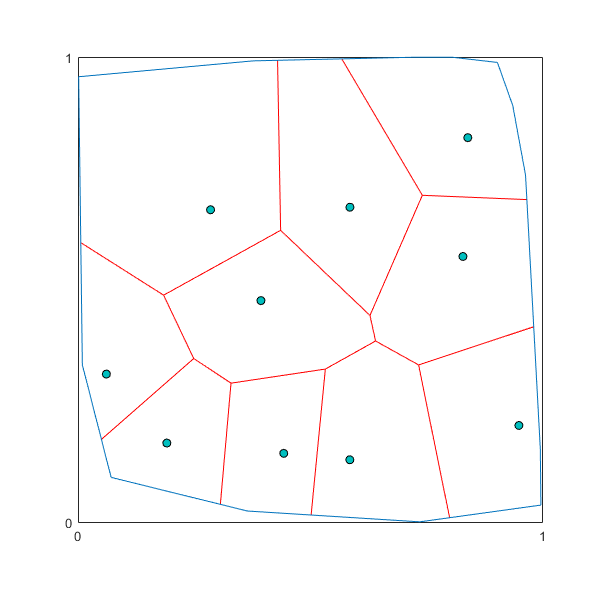
\includegraphics[scale=0.4]{Voronoi-example.png}
\end{center}
\end{frame}

\begin{frame}[label=vorpart2]{Voronoi Partitioning}
While being a method to partition an area with some cost function, the is a widely-used representation in the coverage problem ([Cortes2004][Hussein2007][Du1999])
\\
The Voronoi Diagram of a region $\Omega \subset \rsqr$ is the set of partitions $\mathcal{V} = \left\{V_{i} \mid \cup V_{i} = \Omega\right\}$, generated by the generators $\mathcal{Z} = \{z_1,\ldots,z_n\mid z_{i} \in \Omega\}$, such that
\begin{equation} \label{Voronoi Definition}
V_{i} = \{q\in\Omega \mid \lVert q - z_i \rVert \leq \lVert q - z_j \rVert \forall z_i,z_j\in\mathcal{Z}\},
\end{equation}
where $V_{i}$ corresponds to the $i$-th element of $\mathcal{Z}$, and $\lVert \cdot \rVert$ denotes the Euclidean distance.
\end{frame}

\begin{frame}[label=centvorpart1]{Central Voronoi Tessellations}
And yet again, let's have an intuitive explanation...
\begin{center}
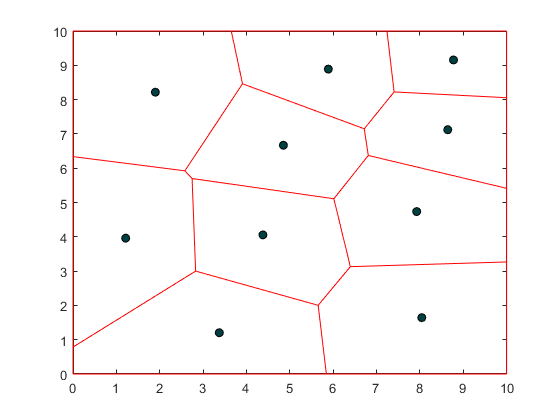
\includegraphics[scale=0.5]{central-Voronoi-example.png}
\end{center}
\end{frame}

\begin{frame}[label=centvorpart2]{Central Voronoi Tessellations}
Let us define a density function, $\rho_i$, for each Voronoi partition $V_{i}$. Then, we can define the center of mass for each partition as
\begin{equation}
z_{i}^{*} = \frac{\int_{V_{i}}y\rho(y)dy}{\int_{V_{i}}\rho(y)dy}.
\end{equation}
If a generator $z_{i} = z_{i}^{*} \, \forall \,V_{i}$, we call this partitioning a \emph{centroidal Voronoi tessellation} (CVT).
\end{frame}

\begin{frame}[label=lloydsalg1]{Lloyd's Algorithm}
Now that we know what Central Voronoi Tessellations are, we need to know how to calculate them. \\
Stuart P. Lloyd, an Electrical Engineer, invented an algorithm that deals with PCM quantization \footnote{Lloyd, S., “Least squares quantization in PCM,” IEEE Transactions on Information Theory, Information Theory, IEEE Transactions on, IEEE Trans. Inform. Theory, Vol. 28, No. 2, 1982, pp. 129–137, doi:10.1109/TIT.1982.1056489}.
\\
It appears that the algorithm is very useful for calculating CVT's. Moreover, It is possible to build a controller based on this algorithm.
\end{frame}

\begin{frame}[label=lloydsalg2]{Lloyd's Algorithm}
\begin{algorithm}[H]
\caption{Lloyd's Algorithm}\label{LloydAlgo}
\begin{algorithmic}[1]
\State Calculate the Voronoi diagram for the current agents positions.
\State Calculate the center of mass for every cell.
\State Move the agents to the center of mass.
\end{algorithmic}
\end{algorithm}
\end{frame}

\begin{frame}[label=lloydsalg3]{Lloyd's Algorithm}
According to Cortes et al., if we define agent $i$ position as $p_i$ and the $i$'s partition centroid as $C_{V_{i}}$, then for some proportional constant $k_{prop}$, the controller can be defined as:
\begin{equation} \label{Lloyds contoller}
u_{i} = -k_{p}\left( p_i - C_{V_{i}} \right)
\end{equation} 
Moreover, this controller is locally asymptotically stable.
\end{frame}

\subsection[Distance-Based Formation Control]{}
\begin{frame}[label=distanceformation1]{Formation Control}
For a complete background, some prior knowledge on algebraic graph theory is needed. Let's simplify:
\begin{itemize}
\item<1-> We have agents $1 \ldots n$ on positions $p_{i}$
\item<2-> We want that the distance between agents $i,j (i \neq j)$ will be $d_{ij}$
\item<3-> Lets assume that there isn't connection between all the agents. Only $\varepsilon$ agents can share information.
\end{itemize}
\end{frame}

\begin{frame}[label=distanceformation2]{Formation Control}
Then, for a single agent $p_i$, the controller will have the following form:
\begin{equation}
    \dot{p_{f_{i}}} = -\sum_{i \sim j} \left( \norm{p_{i} - p_{j}}^{2} - d_{ij}^2 \right) \left( p_{i} - p_{j} \right)
    \label{formation controller}
\end{equation}
This controller is locally asymptotically stable.
\end{frame}

\subsection[Projection Operator]{}
\begin{frame}[label=projoperator]{Projection Operator}

The projection linear operator is defined as a linear transformation $P$ from a vector space to itself such as $P^2 = P$. In other words, the transformation $P$ is idempotent.

\end{frame}

%%%%%%%%%%%%%%%%%%%%%%%%%%%%%%%%%%%%%%%%%%
%%%%%%%%%%%%% PROBLEM SOLUTION %%%%%%%%%%%
%%%%%%%%%%%%%%%%%%%%%%%%%%%%%%%%%%%%%%%%%%

\section[Problem Solution]{Problem Solution}

\subsection[Projected Lloyd's Algorithm]{}
\begin{frame}[label=projlloydsalgo1]{Projected Lloyd's Algorithm}
We should supply a solution for the "Coverage Constraint" \pause
\begin{block}{Reminder}
A given area inside the area $A_{m} \subset A$ must be covered always
\end{block}\pause
We came up with a rather simple solution for this problem.
\end{frame}

\begin{frame}[label=projlloydsalgo2]{Projected Lloyd's Algorithm}
\begin{algorithm}[H]
\caption{Projected Lloyd's Algorithm (PLA)}\label{ProjLloydsAlgorithm}
\begin{algorithmic}[1]
\State Calculate the Voronoi diagram for the current agents positions.
\State Calculate the center of mass for every cell.
\State Project the center of mass of every cell to the area constraint limiting polygon.
\State Move the agents the projected center of mass.
\State Repeat until converge.
\end{algorithmic}
\end{algorithm}

Writing this algorithm as a controller:
\begin{equation} \label{ProjectedLloydsContol}
u_{i} = -k_{p}\left( p_i - \textit{proj}\left( C_{V_{i}} \right) \right)
\end{equation} 
\end{frame}

\begin{frame}[label=projlloydsalgo3]{Projected Lloyd's Algorithm}
In the following example:
\begin{itemize}
\item Left - regular CVT, build with the original Lloyd's Algorithm.
\item Right - A partitioning built with the PLA.
\end{itemize}
\begin{figure}
\centering
\begin{minipage}{.4\textwidth}
  \centering
  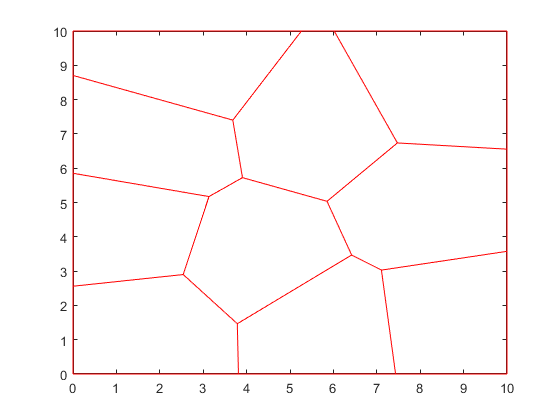
\includegraphics[scale=0.3]{proj-lloyds-off.png}
\end{minipage}
\begin{minipage}{.4\textwidth}
  \centering
  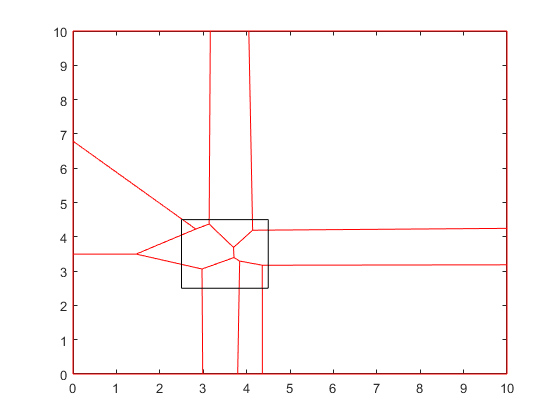
\includegraphics[scale=0.3]{proj-lloyds-on.png}
\end{minipage}
\end{figure}

\end{frame}

\begin{frame}[label=projlloydsalgotheorem]{Projected Lloyd's Algorithm}
\begin{theorem}
The projected Lloyd's Algorithm is locally asymptotically stable
\end{theorem}

As the projection is a linear operator, the controller is also locally asymptotically stable, and the proof is virtually the same as was given by Cortes et al. The proof is based on a proposal of Lyaponov function, and then using the direct Lyaponov method to prove the stability
\end{frame}

\begin{frame}[label=projlloydsalgoproof]{Proof of stability}
As the projection is a linear operator, the controller is also locally asymptotically stable, and the proof is virtually the same as was given by Cortes et al.\\

\end{frame}

\subsection[Problem Solution Algorithm]{}
\begin{frame}[label=probsolalg1]{Problem Solution Algorithm}
So far, we've given solution for:
\begin{itemize}
\item Covering a given area using Voronoi partitioning
\item Partition and area such that the coverage constraint is fulfilled.
\end{itemize}

Therefore, we are ready for the problem solution algorithm...
\end{frame}

\begin{frame}[label=probsolalg2]{Problem Solution Algorithm}
\begin{algorithm}[H]
\caption{Problem Solution Algorithm}\label{GeneralProbSolution}
\begin{algorithmic}[1]
\State Using some random initial guess, partition the whole area using PLA.
\State For each partition (assuming that the agents can actually cover each partition with their coverage radius), calculate the CVT. The initial positions for the CVT calculation is the previous partition CVT.
\end{algorithmic}
\end{algorithm}
\end{frame}

\subsection[Lloyd's Algorithm and Formation Control]{}
\begin{frame}[label=lloydsandformation1]{Lloyd's Algorithm and Formation Control}
\begin{itemize}
\item<1-> Problem solved.
\item<2-> Make it more interesting...
\item<3-> Combine Lloyd's Algorithm with distance-based formation control! \begin{itemize}
\item<4-> create and maintain spatial properties partially or fully (We do not provide a condition where this combination meets the requirements).
\end{itemize}
\end{itemize}
\end{frame}

\begin{frame}[label=lloydsandformation2]{Lloyd's Algorithm and Formation Control}
As both of the controllers are convex, we propose to simply combine them with some coefficient:\\
\begin{equation}
    u_{i} = \alpha \left(-k_{p}\left( p_i -C_{V_{i}} \right)\right) +
    \left( 1-\alpha \right)\left[-\sum_{i \sim j} \left( \norm{p_{i} - p_{j}}^{2} - d_{ij}^2 \right) \left( p_{i} - p_{j} \right)  \right] 
    \label{Combined Controller}
\end{equation}\pause
\begin{theorem}
The combined controller is Locally Asymptotically Stable
\end{theorem}
\end{frame}

\begin{frame}[label=lloydsandformation3]{Lloyd's Algorithm and Formation Control}
How to prove:
\begin{itemize}
\item Pretty long and technical, based on Lyapunov function.
\item We know the Lyapunov function of each controller - Let's combine!
\item After long calculations, we can show using the Lyapunov direct method that this controller is locally asymptotically stable.
\item In the same way, we can show it works with the PLA.
\end{itemize}
\end{frame}



%%%%%%%%%%%%%%%%%%%%%%%%%%%%%%%%%%%%%%%%%%
%%%%%%%%%%%%% Simulations %%%%%%%%%%%
%%%%%%%%%%%%%%%%%%%%%%%%%%%%%%%%%%%%%%%%%%

\section[Simulations]{Simulations}
\subsection[Some Simulation]{}
\begin{frame}[label=sl3]{Some Simulation}
List of simulations to create:
\begin{itemize}
\item 3 agents, 5 big partitions, no formation, no PLA
\item 3 agents, 5 big partitions, no formation, PLA
\item 10 agents, 5 big partitions, no formation, PLA
\item 6 agents, 5 big partitions, some formation, PLA
\end{itemize}
\end{frame}

\end{document}
